%%%%%%%%%%%%%%%%%%%%%%%%%%%%%%%%%%%%%%%%%
% Journal Article
% LaTeX Template
% Version 1.4 (15/5/16)
%
% This template has been downloaded from:
% http://www.LaTeXTemplates.com
%
% Original author:
% Frits Wenneker (http://www.howtotex.com) with extensive modifications by
% Vel (vel@LaTeXTemplates.com)
%
% License:
% CC BY-NC-SA 3.0 (http://creativecommons.org/licenses/by-nc-sa/3.0/)
%
%%%%%%%%%%%%%%%%%%%%%%%%%%%%%%%%%%%%%%%%%

%----------------------------------------------------------------------------------------
%	PACKAGES AND OTHER DOCUMENT CONFIGURATIONS
%----------------------------------------------------------------------------------------

\documentclass[twoside,twocolumn]{article}

\usepackage{blindtext} % Package to generate dummy text throughout this template 

\usepackage[sc]{mathpazo} % Use the Palatino font
\usepackage[T1]{fontenc} % Use 8-bit encoding that has 256 glyphs
\linespread{1.05} % Line spacing - Palatino needs more space between lines
\usepackage{microtype} % Slightly tweak font spacing for aesthetics

\usepackage[english]{babel} % Language hyphenation and typographical rules

\usepackage[hmarginratio=1:1,top=32mm,columnsep=20pt]{geometry} % Document margins
\usepackage[hang, small,labelfont=bf,up,textfont=it,up]{caption} % Custom captions under/above floats in tables or figures
\usepackage{booktabs} % Horizontal rules in tables
\usepackage{graphicx}
\usepackage{lettrine} % The lettrine is the first enlarged letter at the beginning of the text

\usepackage{enumitem} % Customized lists
\setlist[itemize]{noitemsep} % Make itemize lists more compact

\usepackage{abstract} % Allows abstract customization
\renewcommand{\abstractnamefont}{\normalfont\bfseries} % Set the "Abstract" text to bold
\renewcommand{\abstracttextfont}{\normalfont\small\itshape} % Set the abstract itself to small italic text

\usepackage{titlesec} % Allows customization of titles
\renewcommand\thesection{\Roman{section}} % Roman numerals for the sections
\renewcommand\thesubsection{\roman{subsection}} % roman numerals for subsections
\titleformat{\section}[block]{\large\scshape\centering}{\thesection.}{1em}{} % Change the look of the section titles
\titleformat{\subsection}[block]{\large}{\thesubsection.}{1em}{} % Change the look of the section titles

\usepackage{fancyhdr} % Headers and footers
\pagestyle{fancy} % All pages have headers and footers
\fancyhead{} % Blank out the default header
\fancyfoot{} % Blank out the default footer
\fancyhead[C]{Carbon Cars $\bullet$ Vers. I} % Custom header text
\fancyfoot[RO,LE]{\thepage} % Custom footer text

\usepackage{titling} % Customizing the title section

\usepackage{hyperref} % For hyperlinks in the PDF

%----------------------------------------------------------------------------------------
%	TITLE SECTION
%----------------------------------------------------------------------------------------

\setlength{\droptitle}{-4\baselineskip} % Move the title up

\pretitle{\begin{center}\Huge\bfseries} % Article title formatting
\posttitle{\end{center}} % Article title closing formatting
\title{Carbon Cars Final Report} % Article title
\author{%
\textsc{Abdul Ahmed, Adam Filiz, Maverick Ho}\\[1ex] % Your name
\normalsize CMPS 121 \\ % Your institution
\normalsize  Spring 2019
%\and % Uncomment if 2 authors are required, duplicate these 4 lines if more
%\textsc{Jane Smith}\thanks{Corresponding author} \\[1ex] % Second author's name
%\normalsize University of Utah \\ % Second author's institution
%\normalsize \href{mailto:jane@smith.com}{jane@smith.com} % Second author's email address
}
\date{\today} % Leave empty to omit a date
\renewcommand{\maketitlehookd}{%
\begin{abstract}
\noindent Carbon Cars is an application that will allow the user to see how much CO2 they are producing from their vehicle rides. It allows the user to input a type of car for which they will then specify the miles per gallon for said vehicle. Then it will calculate the amount of CO2 created after each trip. A trip is started when the user starts location tracking and then ends when the user stops the location tracking.
\end{abstract}
}

%----------------------------------------------------------------------------------------

\begin{document}

% Print the title
\maketitle

%----------------------------------------------------------------------------------------
%	ARTICLE CONTENTS
%----------------------------------------------------------------------------------------

\section{Objective}

\lettrine[nindent=0em,lines=3]{L} orem ipsum dolor sit amet, consectetur adipiscing elit.
\blindtext % Dummy text

\blindtext % Dummy text

%------------------------------------------------

\section{Components}

When the user first starts the app, they are greeted with the main activity, which consists of a button that starts the location tracker, the logo of carbon cars, as well as a bottom bar navigation. Upon pressing the start button, another activity opens up a list of inputted vehicles that the user has inputted into the app, as well as an edit text view where the user has to input the name of the trip. To start the location tracker, all the user needs to do is to enter a name in the edit text, then press a car from within the list. If the user forgets to put in a name, the location won't start, they have to enter a name, then press a car from the list. To enter a car to the list, the user has to be in the main activity, and press the input cars button within the bottom navigation.
\begin{figure}[h!]
  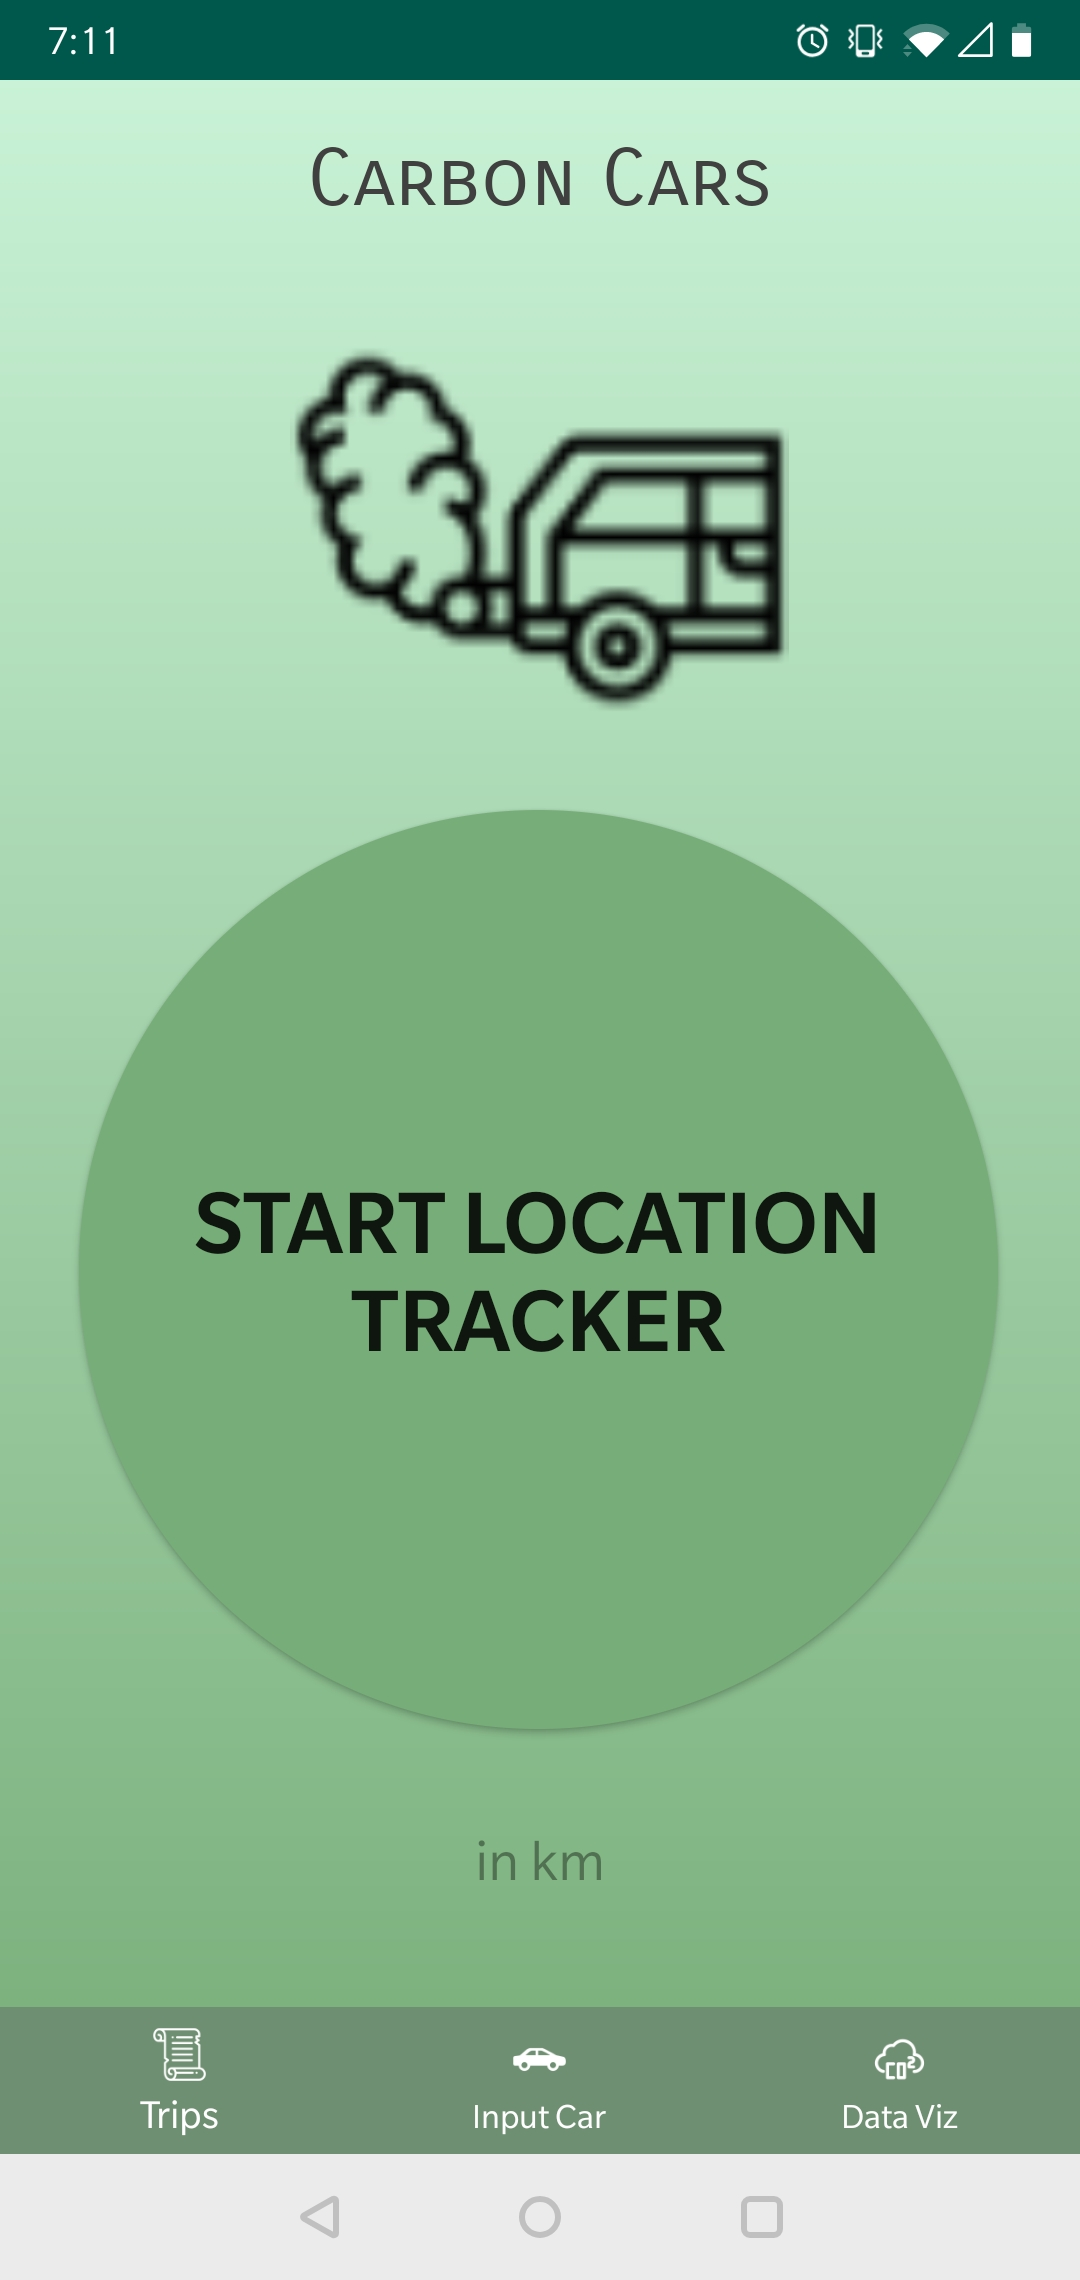
\includegraphics[width=\linewidth,height=14cm,keepaspectratio]{mainscreen.jpg}
  \caption{Screen user is presented with}
  \label{fig:screen}
\end{figure}


In the input cars activity, there is a form that the user fills out. The user can exit out of the form to prevent the location tracker from setting. There are checks to see if a user has filled the form out correctly. Once the user submits a car, they are taken back to the main activity, where the user can now start the location service.

The location service tracks the user, calculating distance traveled. Once the user stops the location tracker, which they can tell because the button has turned red, the data is then recorded into a sqlite database. 

%Probably talk about trip history here.
From there the data from the sqlite database is queried in the Trip History activity that uses an adapter to display and populate the main layout accordingly.We use a RecyclerView since it is versatile for our purpose and added scrolling for better viewing.

%probably talk about your data viz stuff here.
\begin{figure}[h!]
  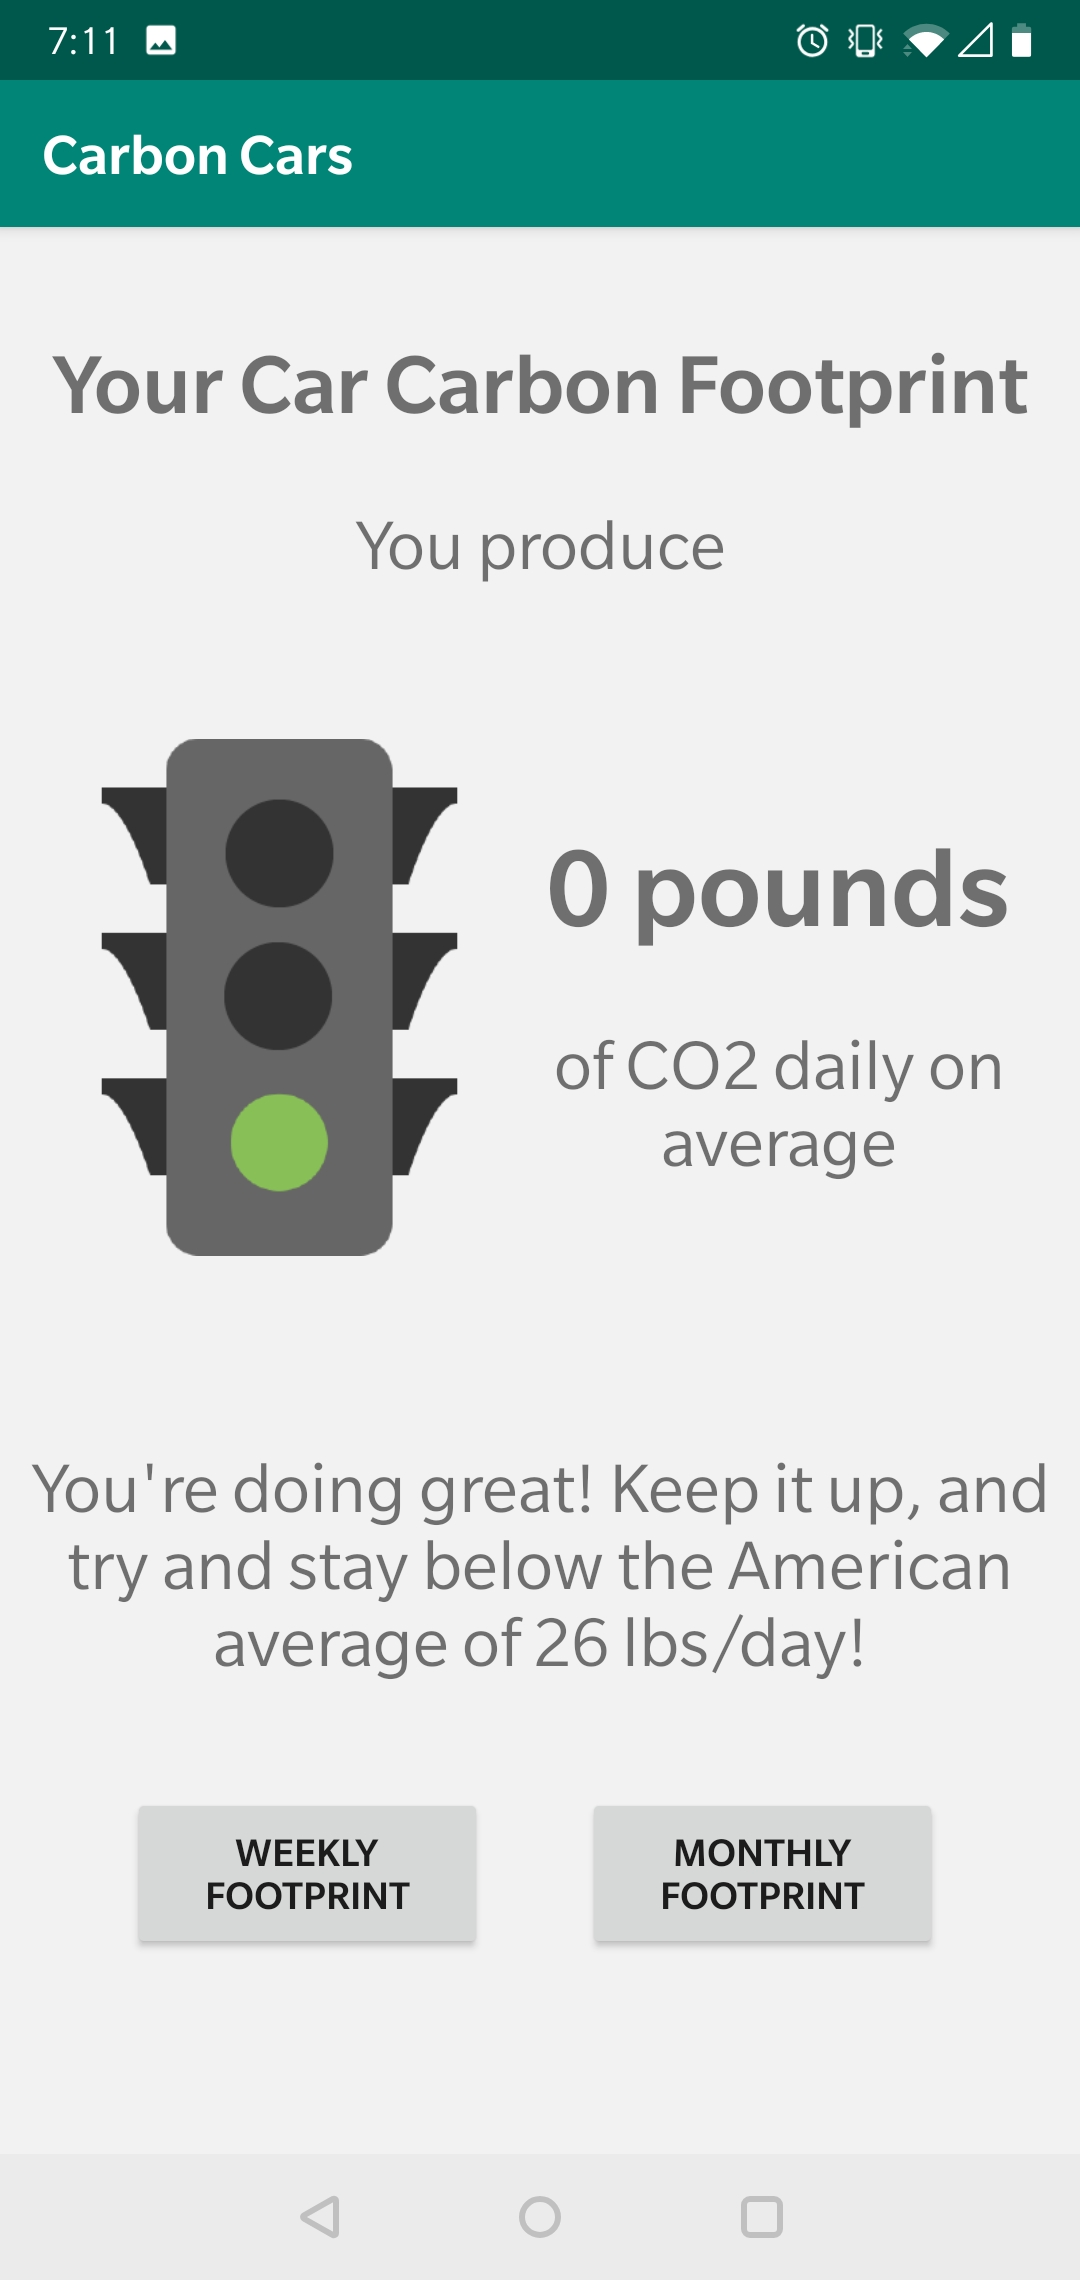
\includegraphics[width=\linewidth,height=14cm,keepaspectratio]{datavis.jpg}
  \caption{Example visual user is greeted with}
\end{figure}
%write data viz stuff here
Blah blah datavis stuff

%------------------------------------------------
\newpage
\section{Development}

The location service was implemented first, since it is the backbone of the project. We knew the main activity had to be the place where the user uses the most. The first order of business was to start a thread that implemented a location listener to track the distance between two points. The thread would receive updates from the location listener whenever the location changed, or if nothing happened within 10 seconds. When updates are received, certain variables within the thread are used. As long as callbacks and updates were not removed from the thread, meaning that the onDestroy function wasn't called, the thread would update values given to it by the location listener. When the onDestroy method was finally called, the thread would have a value called distance, in which kept track of the total distance traveled. The thread would then calculate the amount of CO2 used with a function. The thread communicates with the main activity with a local broadcast, sending information if the thread was explicitly called to stop, or destroyed.

Most of the implementation for the location service hasn't changed from its intended use. Only a few changes were added, such as inquires to the user for location access, as well as how to implement the start/stop service button. Initially we wanted the user to start the location dynamically, meaning the app would automatically detect speed of movement using some sort of accelerometer. This was troublesome to implement, since it meant a thread would have to be bonded to the main activity, and kept running while the app was alive. Integrating that functionality was too much of a challenge, and we decided to keep it how it was.

The input cars activity was just meant to be a simple form where the user could enter in information about their car. The activity communicates with the main activity using data passed through intents. Within the activity are functions to check whether of not a user has correctly filled out the form ie: is the a name for the car, are the radio buttons selected within the radio button group, is the mpg even a number?

In order for the various activities to store and use data, a sqlite database class was created in order to facilitate this. Thus a reference to  the the class is initialized in each class, which all use the class functions to help insert/get data. Currently there is only insertion functions as well as getter functions that return cursors based on selection. A few more functions, such as updating or clearing the database would've be nice. 

The trip history pages uses the sqlite database to populate the Trip History layout with all of the trips that the user has initiated.


\section{Logo Citations}
\begin{itemize}
\item All bottom navigation logos are made/taken from freepik.com
\item Logo Icon made by https://www.flaticon.com/authors/darius-dan.
\end{itemize}
%------------------------------------------------

\section{Contribution}

\subsection{Maverick's Contribution}
I implemented main functionality of the location service, calculation of distance/C02, input cars activity, the database wrapper class, and the bottom navigation - including the interaction between the activities. Additionally I helped with the UI on a small scale, as well as planning how the activities should interact with each other.

I would say the app is around eighty percent done. There are still bugs, as explained in the future work reference, as well as some features that we want to implement. 

\subsection{Adam's Contribution}


\subsection{Abdul's Contribution}
I implemented the "Trip History" page so that any data from the User is automatically updated in the trip history page so that they can see how many miles they traveled, amount of emissions, date and other useful tidbits of information for the user to know. I helped around with other parts such as U/I suggestions and gave my input when necessary.
%----------------------------------------------------------------------------------------
%	REFERENCE LIST
%----------------------------------------------------------------------------------------
\section{Future Work}
There are some known bugs. Currently, if a user inputs a car name with an apostrophe, the insertion will not be valid. Additionally, if the app is exited, the thread will stop running... which is not supposed to happen.

Some future work that would be useful for the app would be a more detailed report when the User clicks on a trip in the trip history page.
%----------------------------------------------------------------------------------------

\end{document}
